% Created 2016-08-17 Wed 14:38
\documentclass[tikz]{standalone}

\usepackage[utf8]{inputenc}
\usepackage[T1]{fontenc}

\usepackage{circledsteps}

\RequirePackage{xcolor}

%% HPI color definitions according to the design manual
% These do not exactly match the RGB values used in the Powerpoint slide master due to unknown reasons
\definecolor{hpiyellow}{RGB}{246,168,0}
\definecolor{hpiorange}{RGB}{221,97,8}
\definecolor{hpired}{RGB}{177,6,58}
\definecolor{hpigray}{RGB}{90,96,101}
\definecolor{hpiblue}{RGB}{0,122,158}


\renewcommand{\sfdefault}{neosans}
% Different font weights for neosans
\newcommand{\textl}[1]{{\fontseries{l}\selectfont #1}} % light
\newcommand{\textm}[1]{{\fontseries{m}\selectfont #1}} % medium, same as default weight
\newcommand{\textsb}[1]{{\fontseries{sb}\selectfont #1}} % semibold
\newcommand{\textmb}[1]{{\fontseries{mb}\selectfont #1}} % bold, same as \textbf
\newcommand{\texteb}[1]{{\fontseries{eb}\selectfont #1}} % extra bold
\newcommand{\textub}[1]{{\fontseries{ub}\selectfont #1}} % ultra bold

\tikzset{every picture/.style={/utils/exec={\sffamily}}}
\tikzset{flipflop RSflanke/.style={
  flipflop,
  flipflop def={t1=S, t2=C, c2=1, t3=R, t6=Q, t4={\ctikztextnot{Q}}}
}}


\tikzset{
  mechanicalSwitch/.pic={
    \coordinate (-inUp) at (135:2); 
    \coordinate (-inDown) at (235:2);
    \coordinate (-out) at (2,0);
    \coordinate (-center) at (0,0);
    
    \draw (0,0) circle [radius = 2cm];
    \draw [fill=gray!20] (0,0) circle [radius = 0.2cm];

    \draw (0, 0) -- (2, 0);
    \draw (135:.8) -- (135:2); 
    \draw (225:.8) -- (225:2); 

    \draw [fill=gray!20] (2, 0) circle [radius=0.05cm]; 
    \draw [fill=gray!20] (135:2) circle [radius=0.05cm]; 
    \draw [fill=gray!20] (225:2) circle [radius=0.05cm]; 

    
    \draw [thick] (0,0) -- (175:1.5); 

    \draw [dashed, <->, domain=135:225] plot ({cos(\x)}, {sin(\x)}); 
  },
  mechanicalSwitchClosed/.pic={
    \coordinate (-inUp) at (135:2); 
    \coordinate (-inDown) at (255:2);
    \coordinate (-out) at (2,0);
    \coordinate (-center) at (0,0);
    \draw (0,0) circle [radius = 2cm];
    \draw [fill=gray!20] (0,0) circle [radius = 0.2cm];

    \draw (0, 0) -- (2, 0);
    \draw (135:.8) -- (135:2); 
    \draw (225:.8) -- (225:2); 

    \draw [fill=gray!20] (2, 0) circle [radius=0.05cm]; 
    \draw [fill=gray!20] (135:2) circle [radius=0.05cm]; 
    \draw [fill=gray!20] (225:2) circle [radius=0.05cm]; 

    
    \draw [thick] (0,0) -- (135:2); 

    \draw [dashed, <->, domain=135:225] plot ({cos(\x)}, {sin(\x)}); 
  }
}


\usetikzlibrary{calc}
\usetikzlibrary{positioning}



\usetikzlibrary{decorations.pathreplacing}


\begin{document}

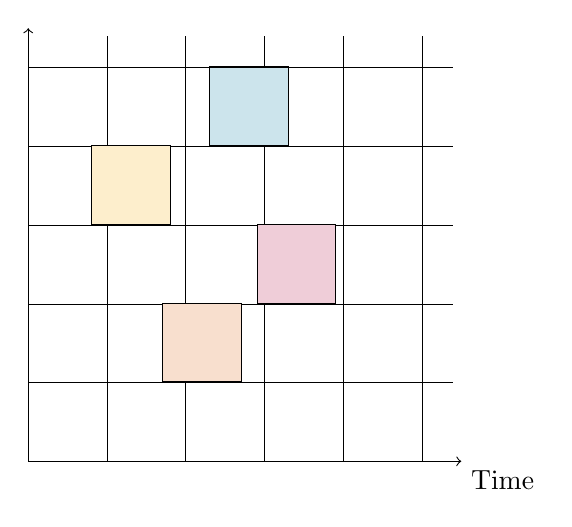
\begin{tikzpicture}
  \label{page:mac:continuous_time}
  \draw [very thin] (0,0) grid (5.4,5.4); 
  \draw [->] (0,0) edge (0,5.5) -- (5.5,0) node[below right] {Time};

  \begin{scope}[every node/.style={minimum width=1cm, minimum height=1cm, anchor=south west, draw}]
    \node [fill=hpiyellow!20, ] at (0.8, 3) {}; 
    \node [fill=hpiorange!20, ] at (1.7, 1) {}; 
    \node [fill=hpiblue!20, ] at (2.3, 4) {}; 
    \node [fill=hpired!20, ] at (2.9, 2) {}; 
  \end{scope}

\end{tikzpicture}


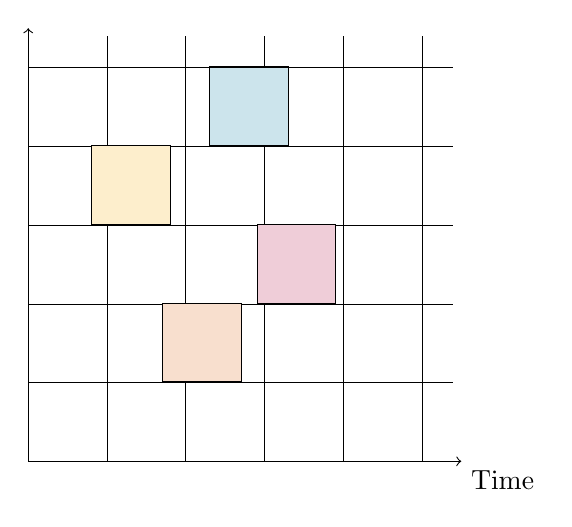
\begin{tikzpicture}
  \label{page:mac:slotted_time}

  \draw [very thin] (0,0) grid (5.4,5.4); 
  \draw [->] (0,0) edge (0,5.5) -- (5.5,0) node[below right] {Time};

  \begin{scope}[every node/.style={minimum width=1cm, minimum height=1cm, anchor=south west, draw}]
    \node [fill=hpiyellow!20, ] at (0.8, 3) {}; 
    \node [fill=hpiorange!20, ] at (1.7, 1) {}; 
    \node [fill=hpiblue!20, ] at (2.3, 4) {}; 
    \node [fill=hpired!20, ] at (2.9, 2) {}; 
  \end{scope}

\end{tikzpicture}

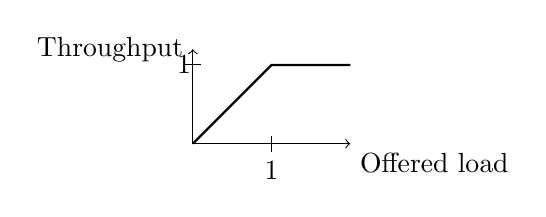
\begin{tikzpicture}
  \label{page:mac:ideal_throughtput}
  \draw [->] (0,0) -- (0,1.2) node [left] {Throughput};
  \draw [->] (0,0)  -- (2,0) node[below right] {Offered load};
  \draw (1,0.1) -- (1,-0.1) node [below] {1}; 
  \draw (-0.1,1) -- (0.1,1) node [left] {1}; 
      
  \draw [thick] (0,0) -- (1,1) -- (2,1); 
\end{tikzpicture}



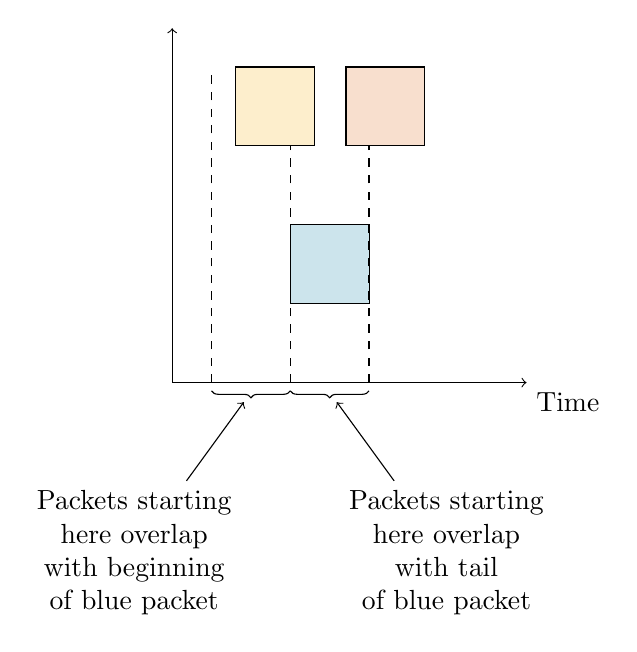
\begin{tikzpicture}
  \label{page:mac:vulnerable}
  % \draw [very thin] (0,0) grid (4.4,4.4); 
  \draw [->] (0,0) edge (0,4.5) -- (4.5,0) node[below right] {Time};

  \begin{scope}[every node/.style={minimum width=1cm, minimum height=1cm, anchor=south west, draw}]
    \node [fill=hpiyellow!20, ] at (0.8, 3) {}; 
    \node [fill=hpiorange!20, ] at (2.2, 3) {}; 
    \node [fill=hpiblue!20, ] at (1.5, 1) {}; 

    \draw [dashed] (0.5, 0) -- (0.5,4); 
    \draw [dashed] (1.5, 0) -- (1.5,3); 
    \draw [dashed] (2.5, 0) -- (2.5,3);

  \end{scope}

  \draw [decorate, decoration={brace,mirror,raise=3pt}] (0.5, 0) to node[below=0cm, align=center] (ll) {} (1.5,0); 

  \node [below left=1cm and 0cm of ll, align=center] (lll) {Packets starting \\here overlap \\with beginning \\of blue packet}; 


  \draw [decorate, decoration={brace,mirror,raise=3pt}] (1.5, 0) to node[below=0cm, align=center] (rl) {} (2.5,0); 

  \node [below right=of ll, align=center] (rll) {Packets starting \\here overlap \\with tail  \\of blue packet}; 

  \draw[->] (rll) -- (rl); 
  \draw[->] (lll) -- (ll); 
\end{tikzpicture}



\end{document}